%% 情報学群実験第3,4(C)用のレポートテンプレート
%
\documentclass[a4j,titlepage]{jarticle}
%% プリアンブルここから
\usepackage[dvipdfmx]{graphicx}
\usepackage{url}
\usepackage{comment}
%
\title{\huge 配達支援システム\\
		外部設計書}
\author{第0版\\
        ONO-Systems\\}
\date{\today}

%本文
\begin{document}
\maketitle

%目次
\tableofcontents
\clearpage

\section{目的}
現在,日本で行われている形態の宅配便サービスが開始し,約40年ほど経過しています.近年のECサイトの拡大に伴い,食料品や日用雑貨などを購入する利用者も増えており,ネットショッピングは特別な商品を買う場所ではなく,近所への買い物と似たような感覚で利用する人々が増えているため,宅配便の取扱個数はさらなる増加が予想されます\cite{ref1}.\\
\ \ \ その一方で,全体の取扱個数の中でも約2割ほどが再配達になっており,さらに約4割の利用者が「配達されることを知らなかった」という調査結果が国土交通省の調査により明らかになっています(図2).この2割にのぼる再配達を労働力に単純に換算すると年間約9万人もの労働力に相当するとも言われています.また,再配達によりトラックなどから排出される二酸化炭素によって,地球温暖化問題にも影響を与えています.さらに,再配達と宅配便の取扱個数の増加により,配達員の長時間労働などの問題が生じ,配達員の人手不足も深刻になっています\cite{ref1}.\\
\ \ \ 利用者側からすると商品が届いて不在票をもらう前に,利用者側から容易に配達員に受け取りの可否を連絡することは難しいです.\\
%=====================================
\ \ \ そこで,弊社では情報技術を駆使することにより宅配業務における配達員の負担を軽減し,消費者の利便性にも配慮した配達支援システムを提案します.
%=====================================

\section{システム概要}
ここでは,システムの機能概要を説明します.

\subsection{サブシステムの概要}
本システム内を構築するためのサブシステムの概要を以下に示します.

\subsubsection{位置情報通知サブシステム}
配達員が利用者の住所に近づいた場合またはトラックに荷物を運びこむ営業所の時点で,配達員の位置情報を受信できます.

\subsubsection{配達物の受け取り可否選択サブシステム}
利用者は配達物の受け取り可否を選択することができ,その選択結果は配達員に送信されます.

\subsubsection{音声読み上げサブシステム}
配達員は,受け取り可能な利用者の名前と住所を合成音声で読み上げさせることができます.

\subsubsection{受け取り可否の地図上表示サブシステム}
配達員は,受け取り可能な利用者の名前や住所,時間帯を地図上にプロットして色などから情報を判断することができます.

\subsection{サブシステムの詳細}
サブシステムの詳細を以下に示します.

\subsubsection{位置情報通知サブシステム}
入力:\\
出力:\\
処理:

\subsubsection{配達物の受け取り可否選択サブシステム}
入力:\\
出力:\\
処理:

\subsubsection{音声読み上げサブシステム}
入力:\\
出力:\\
処理:

\subsubsection{受け取り可否の地図上表示サブシステム}
入力:\\
出力:\\
処理:


\section{利用者インタフェース設計書}
ここでは,利用者が用いる際に使用するユーザインターフェースの設計を示します.

\subsection{画面遷移図}
あとは「社長」と「東」にまかせた...




\section{システムのハードウェア構成}
本システムのハードウェア構成は表1の通りです.
\begin{table}[htbp]
\begin{center}
 \caption{ハードウェア構成}
  \begin{tabular}{|c|c|}\hline
    項目 & 数量 & 備考\\ \hline \hline
    サーバ & 1台 & AWS\\ \hline
    管理者端末 & 1台 & \\ \hline
  \end{tabular}
\end{center}
\end{table}


\section{ソフトウェア構成}
システム間のやり取りは,Java,MySQLを用いて行います.

\section{データテーブル設計書}
ここでは,データベースを構築する MySQL のデータベース構築,データベースの仕様を定義します.

\subsection{データベース構築}
ER図とか

\subsection{データテーブル仕様}
本システムではサーバで使用するデータベースとして以下のテーブルを定義します.なお,アンダーラインの項目は主キーを表します.

\subsubsection{Aテーブル}
\subsubsection{Bテーブル}



\section{ネットワーク構成}
本システム全体のネットワーク構成を以下の図に示します.

\begin{figure}[htbp]
 \begin{center}
  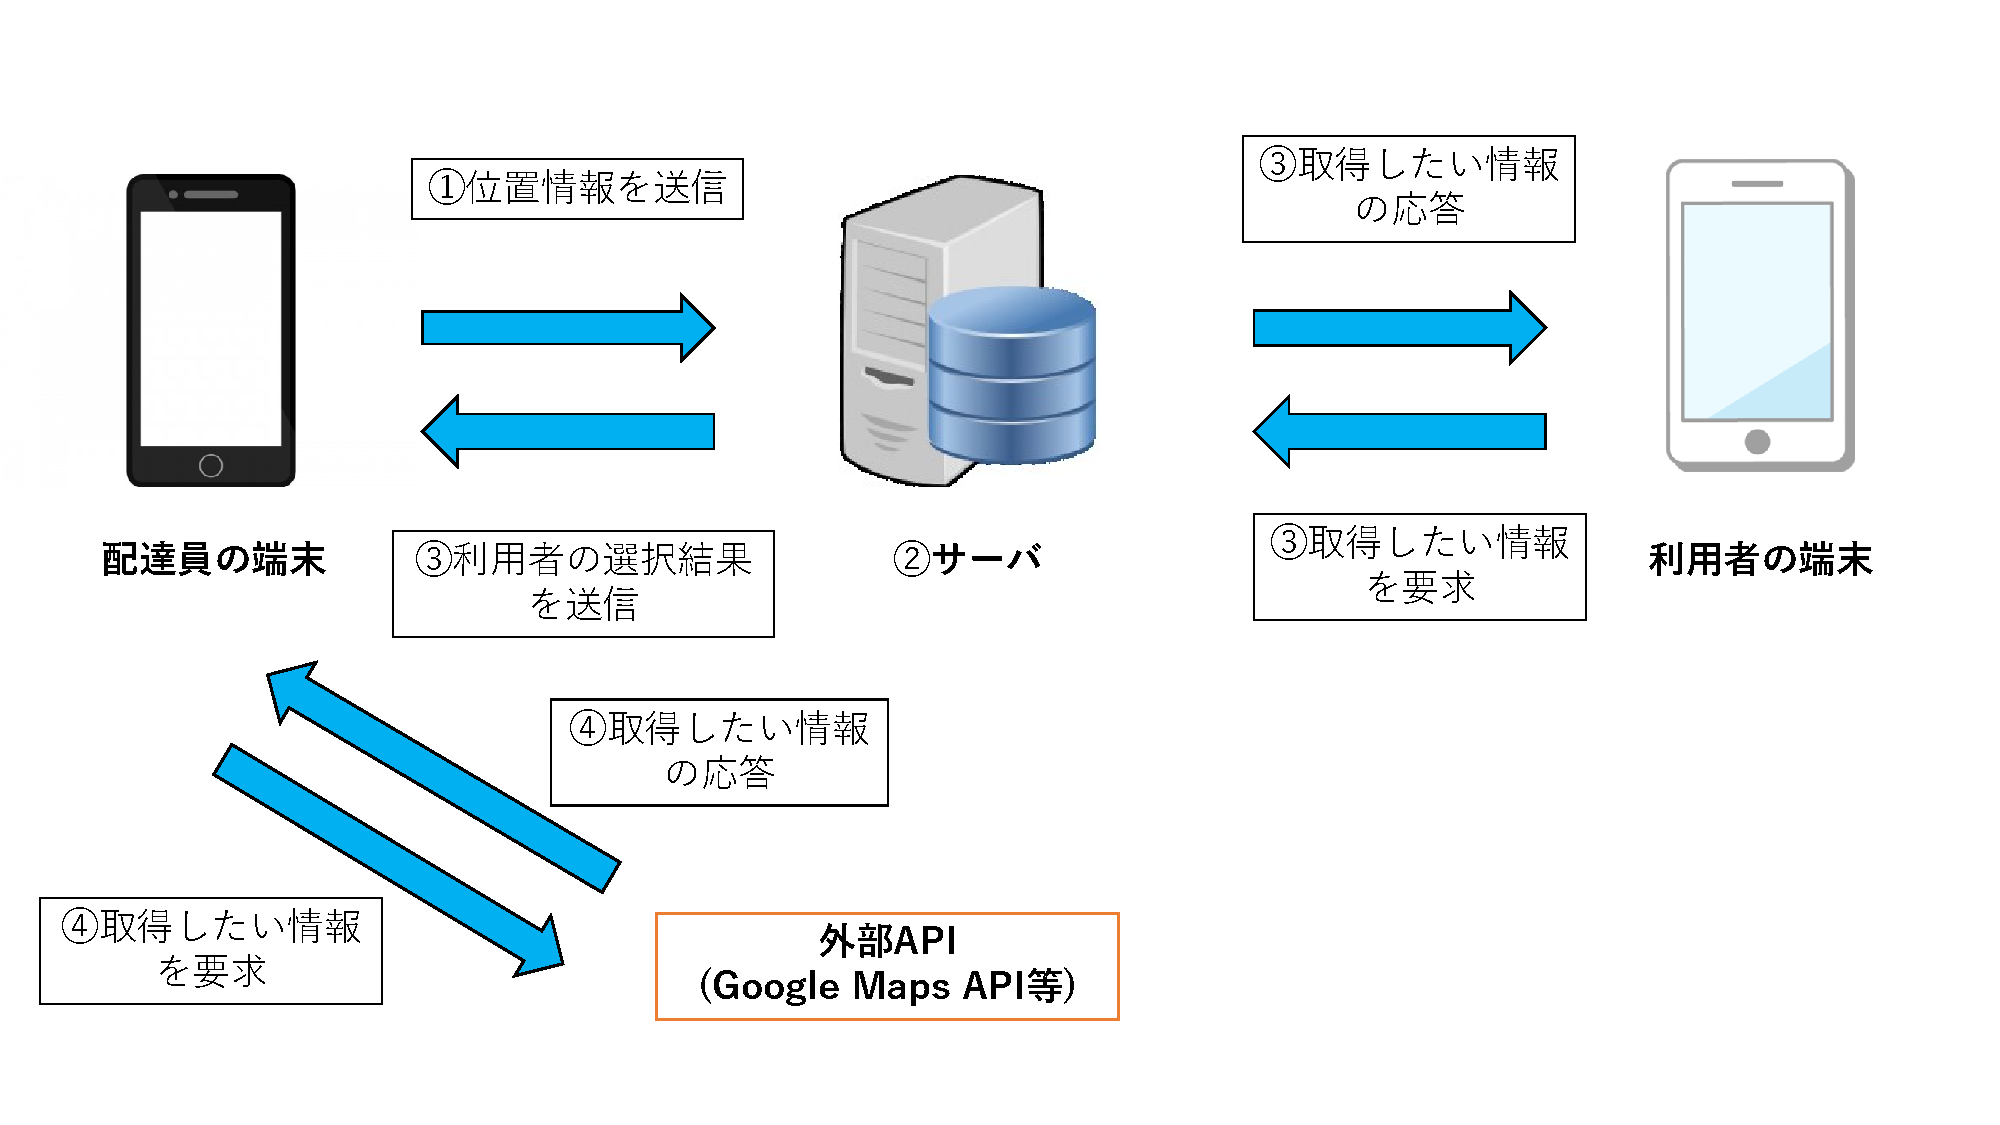
\includegraphics[width=140mm]{情報の流れ.pdf}
 \end{center}
 \caption{情報の流れ}
\end{figure}


\section{ネットワーク接続形態}
本システムでは利用者端末,管理者端末は TCP/IP を用いてサーバと通信を行います.


\section{用語の定義}
本システムでは以下のように用語を定義します.
\begin{itemize}
 \item 利用者:ネットショッピングなどを通じて商品を購入して,自宅に配送するように指定した消費者
 \item 配達員:宅配業者の従業員で商品をお客様の家まで届ける人
\end{itemize}

\begin{thebibliography}{9}

\bibitem{ref1}
国土交通省,
\newblock ``宅配便の再配達削減に向けて'',\\
\newblock \url{http://www.mlit.go.jp/seisakutokatsu/freight/re_delivery_reduce.html}, \\
2018/10/11
\bibitem{ref2}
エン・ジャパン株式会社,
\newblock ``ヤマト運輸株式会社 中部支社のドライバー ★平均月収35万円。無理なく年収400万円が見込めます。'',\\
\newblock \url{https://employment.en-japan.com/desc_770664/}, \\
2018/10/11
\end{thebibliography}

\end{document}
